\newcommand{\todo}[1]{{\bf TODO} #1}
\newif\ifPAPER  
%\PAPERtrue % select either slide or note
\PAPERfalse  

\def\t{\title{Comparison of NIRS HIMAC and HIBMC $^{12}$C beam data with Geant4 simulation} }

\def\a{
\author{A.~Heikkinen} 
\affiliation{Helsinki Institute of Physics, P.O. Box 64, FIN-00014 University of Helsinki (Finland)}
}

\newcommand{\codeAlgorithm}[1]{
\addcontentsline{toc}{section}{Résumé}
\begin{center}\fbox{\parbox{12cm}{\bf #1}}\end{center}}

\newcommand{\cppintro}[1]{
\lstset{language=C,
caption= #1 ,
label=listing:boundary}}

\def\cppstart{\begin{lstlisting}}
\def\cppend{\end{lstlisting}}

\newif\ifCITENOTE 
\CITENOTEtrue

\ifPAPER

\else   % Slides ---------------------------------------------------------------

\documentclass[slidestop,compress,xdvips,10pt]{beamer} 
\usetheme{Antibes}
\usecolortheme{lily}
\usepackage{graphicx}
\usepackage{hyperref}
\usepackage{listings}
\usepackage{verbatim} % for comment
\transglitter[direction=315]
\xdefinecolor{ahcol}{rgb}{0.2, 0.4, 0.1}
\xdefinecolor{olive}{cmyk}{0.64,0,0.95,0.4}
\colorlet{structure}{green!60!black} % for color substitution
\usepackage{color} % for definecolor
\definecolor{light-gray}{gray}{0.95}
\definecolor{dark-gray}{gray}{0.30}
\definecolor{orange}{rgb}{1,0.5,0}
\definecolor{dark-blue}{cmyk}{1,0.5,0.5,0}
\usepackage{attachfile} 
\hypersetup{
    a4paper, % page format
    pdftitle={My Title},                  % Title
    pdfsubject={Subject of the document}, % Subject 
    pdfauthor={Author name},              % Author
    pdfkeywords={list of keywords},       % Keywords
    plainpages=true, %
    colorlinks,       % links are colored
    urlcolor=dark-blue,    % color of external links
    linkcolor=dark-blue,    % color of internal links
    citecolor=black,  % color of links to bibliography
    bookmarksnumbered
}

\usecolortheme[named=ahcol]{structure}
\useoutertheme{myinfolines}
\useinnertheme{rounded}
\setbeamercolor{alerted_text}{fg=blue}

\makeatother
\beamertemplatetransparentcoveredhigh
\t
\author{\underline{A.~Heikkinen} (on behalf of Takashi Sasaki and Toshiyuki Toshito)
\footnote{Helsinki Institute of Physics, P.O. Box 64, FIN-00014 University of Helsinki, Finland.
aatos.heikkinen@cern.ch}}

%\author{Aatos Heikkinen 
%\footnote{Helsinki Institute of Physics, Helsinki, Finland.
%%{\tt aatos.heikkinen@cern.ch}} and Ivica Puljak 
%\footnote{University of Split - FESB, Split, Croatia}
%}
\graphicspath{{.}{figures/}}
\graphicspath{{images/}}
\begin{document}

%\begin{comment}
\frame{\titlepage}
%\end{comment}

\section{}

\subsection{}
\frame{
\frametitle{Summary of Geant4 talks in the 2nd RCM}
Geant4 talks in 2nd RCM of the Coordinated Research Project (CRP):
\begin{itemize}
\item Suitability of Bertini, Binary and other models for simulation of proton induced 
Bragg peak. (H.~Paganetti)
\item Details of Binary (including light ions) and Bertini cascade. 
Latest results from data libraries. (J.~M.~Quesada)
\item Functionality of Hadrontherapy example. Suggestion for further development: 
Benchmarking platform for the CRP. (G.A.P.~Cirrone, G.~Cuttone, F.~Romano, {\em et al.})
\item Suggestion to consider a new Geant4 model INCL in the CRP. (A.~Heikkinen)  
\item Note from the Japanese team. (A.~Heikkinen for the Japanese team in these slides)
\begin{itemize}
\item Slides were provided by Takashi Sasaki and Toshiyuki Toshito introduce
the tuning of Geant4 EM models for the best reproduction of the Bragg peak parameters. 
\item There has been a close collaboration with V.~Ivanchenko and S.~Incerti. 
\item The results are due to extensive work by Geant4 EM developers, and the Japanese team.
\end{itemize}

%Toshiuki has been working in close touch with Vladimir and Sebastien, 
%and they can also inform you about EM developments.  


\end{itemize}
}

\frame{
\frametitle{}
\vspace{0.1cm}
\begin{center}
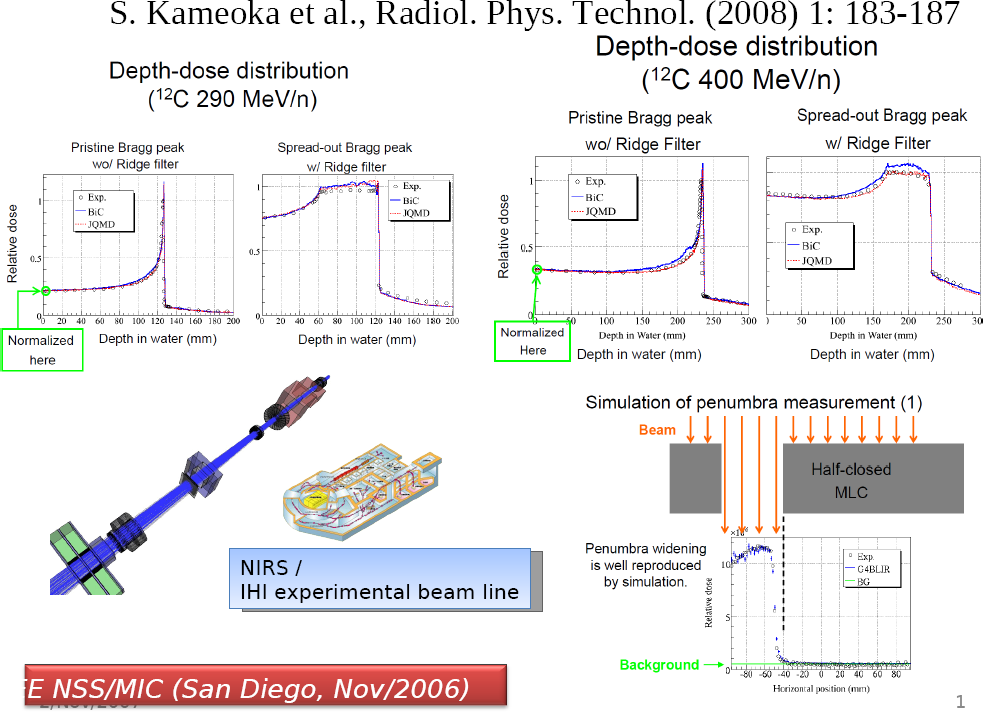
\includegraphics[width=0.95\textwidth]{jp1}
\end{center}
}

\frame{
\frametitle{}
\vspace{0.1cm}
\begin{center}
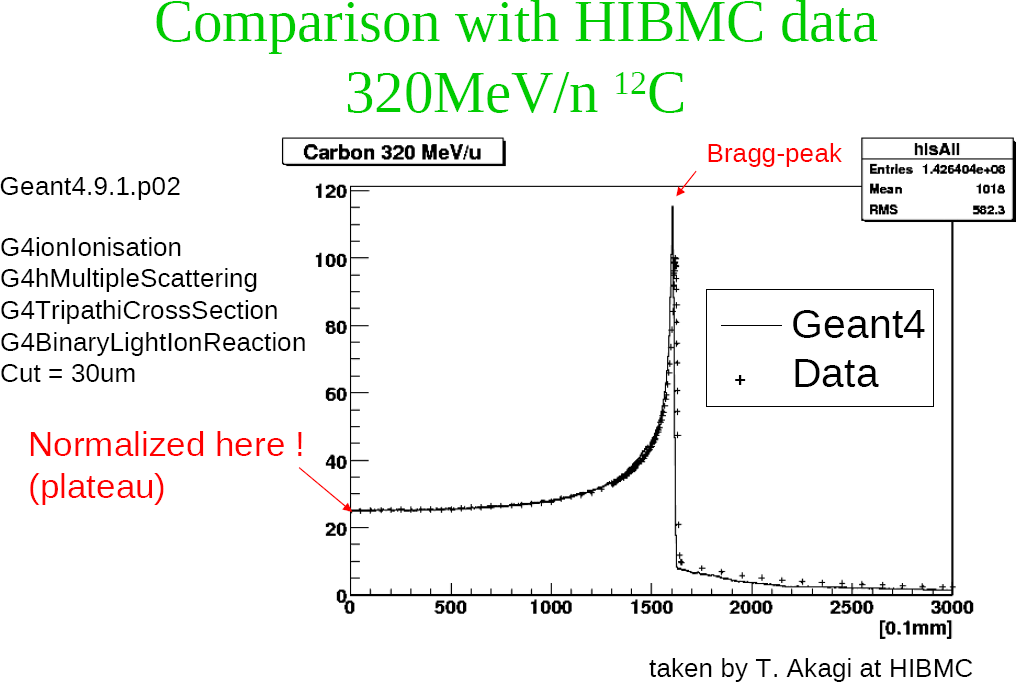
\includegraphics[width=1.00\textwidth]{jp2}
\end{center}
}

\frame{
\frametitle{}
\vspace{0.1cm}
\begin{center}
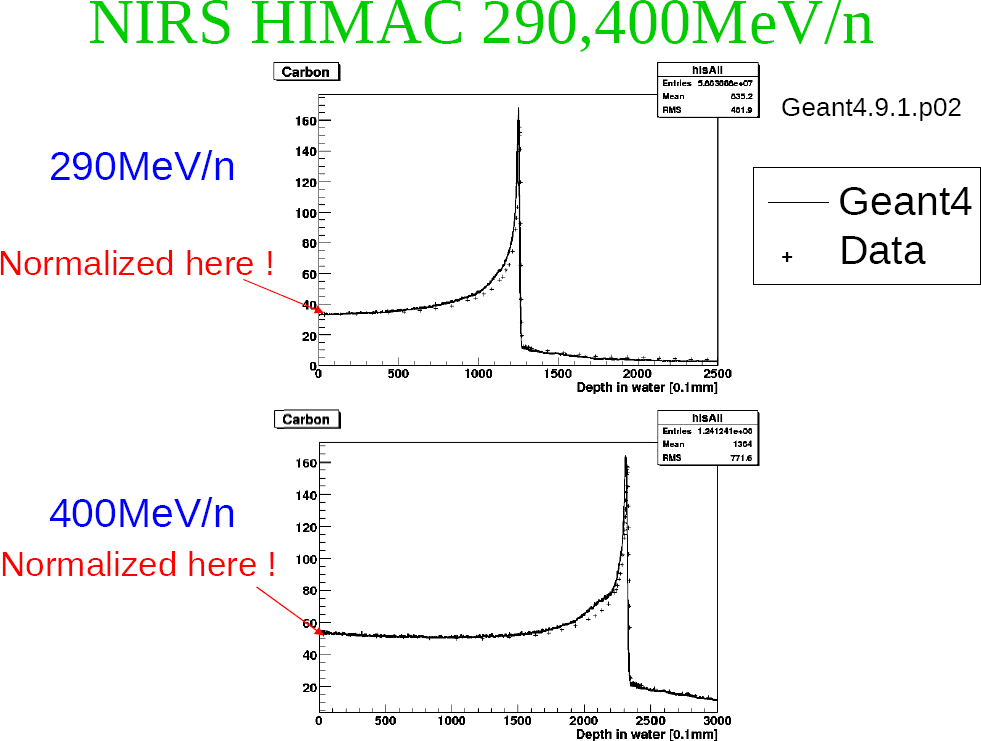
\includegraphics[width=0.91\textwidth]{jp3}
\end{center}
}

\frame{
\frametitle{}
\vspace{0.1cm}
\begin{center}
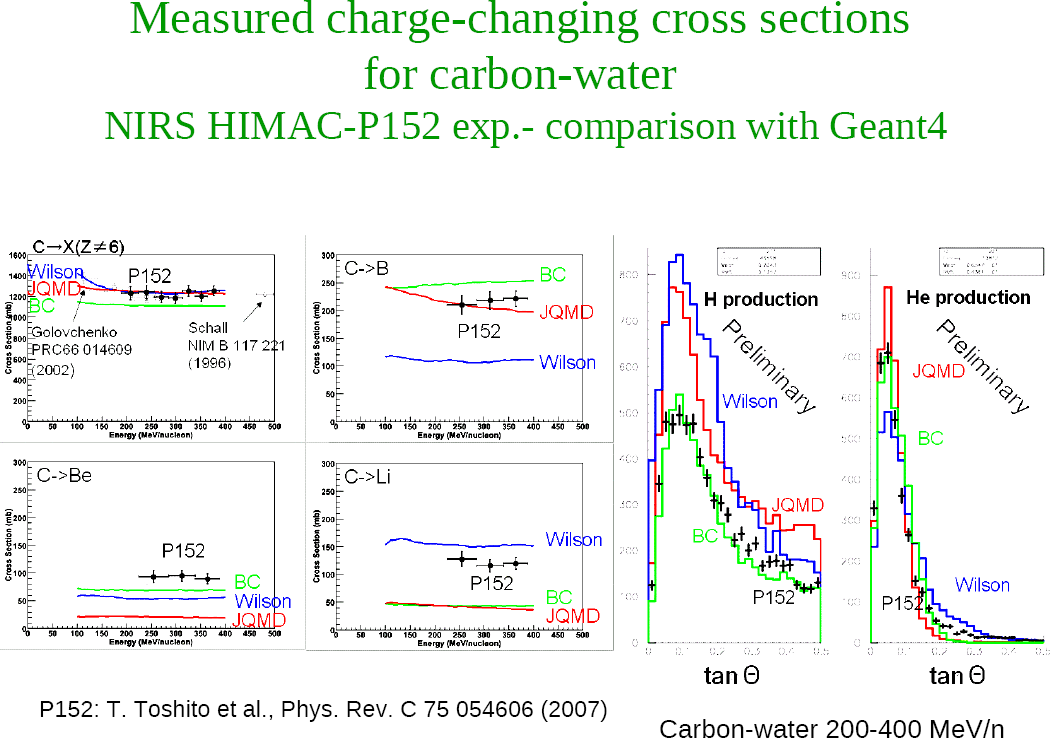
\includegraphics[width=0.95\textwidth]{jp4}
\end{center}
}


%\begin{frame}[allowframebreaks]{References}
%\bibliographystyle{alpha}  % Options plain, unsrt, alpha, abbrv
%\bibliography{refs} %10 p
%\end{frame}
\end{document}

\fi %slides



